\section{Durchführung}
\label{sec:Durchführung}
Die Dampfdruckkurve wird anhand von Messungen im Bereich von $30\,\unit{\milli\bar}$ bis $15000\, \unit{\milli\bar}$ bestimmt.
Dafür werden die Messungen des niedrigen Bereichs (unter $1000\, \unit{\milli\bar}$) und des hohen Bereichs (über $1000\, \unit{\milli\bar}$)
mit zwei verschiedenen Apparaturen durchgeführt.
\subsection{Messbereich von 30\,mbar bis 1000\,mbar}
\label{sec:ErsteDurchführung}
\begin{figure}[H]
    \centering
    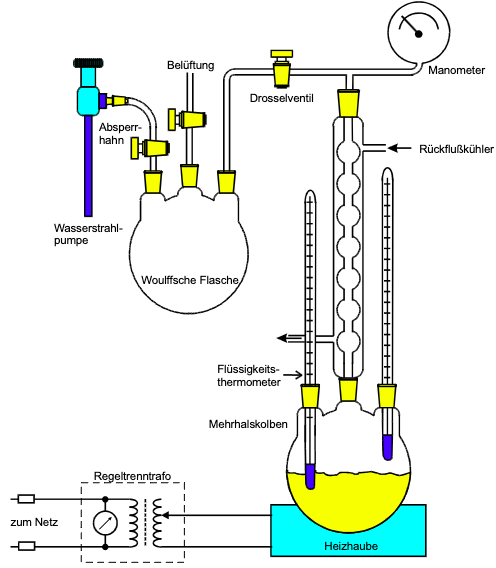
\includegraphics[width=0.60\textwidth]{Erste_Apparatur.png}
    \caption{Skizze der Messapparatur für den Druckbereich $p<1\,\unit{\bar}$. \cite{anleitungV203}}
    \label{fig:ErsteApparatur}
\end{figure}
Um die Dampfdruckkurve von Wasser zwischen $30\,\unit{\milli\bar}$ und $1000\,\unit{\milli\bar}$ zu bestimmen, wird die in Abbildung
(\ref{fig:ErsteApparatur}) zu erkennende Apparatur verwendet. Zunächst wird die Wasserstrahlpumpe evakuiert. Hierfür müssen die Belüftungsventile geschlossen sein, während der Absperrhahn
und das Drosselventil geöffnet sind. Sobald der Druck sich dem niedrigsten Druck angenähert hat, ist der Enddruck erreicht.  
Anschließend wird der Absperrhahn, das Drosselventil und die Wasserstrahlpumpe geschlossen. Damit beim Abstellen der Leitungswasserzufuhr kein kaltes Wasser in die
evakuierte Apparatur eindringt, ist die Woulffsche Flasche vorhanden. Zusätzlich sollte vor dem Abstellen der Wasserstrahlpumpe zunächst der Absperrhahn geschlossen werden.
Daraufhin wird der mit Wasser befüllte Mehrhalskolben mithilfe der Heizhaube erhitzt. Gleichzeitig wird die Kühlwasserzufuhr eingeschaltet. Nach der Anheizzeit siedet das Wasser.
Für die Messung wird für mehrere Temperaturen $T$, in einem Abstand von $1\,\unit{\celsius}$, der jeweilige Druck $p$ mit dem Manometer gemessen bis eine Temperatur von $T= 100\,\unit{\celsius}$ erreicht ist.
Während der gesamten Durchführung muss darauf geachtet werden, dass der Kühlwasserdurchfluss konstant tropft.
\subsection{Messbereich von 1\,bar bis 15\,bar}
\label{sec:ZweiteDurchführung}
\begin{figure}[H]
    \centering
    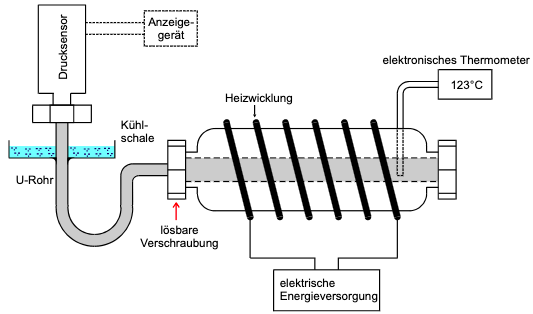
\includegraphics[width=0.70\textwidth]{Zweite_Apparatur.png}
    \caption{Skizze der Messapparatur für den Druckbereich $p>1\,\unit{\bar}$. \cite{anleitungV203}}
    \label{fig:ZweiteApparatur}
\end{figure}
Den Verlauf der Dampfdruckkuve im Druckbereich von $1\,\unit{\bar}$ bis $15\,\unit{\bar}$ wird mit der Apparatur bestimmt, die in Abbildung (\ref{fig:ZweiteApparatur}) zu sehen ist. 
Diese besteht aus einem durcbohrten Stahlbolzen. In dem Hohlraum des Stahlbolzen befindet sich das Wasser, was durch die Heizwicklung um den Stahlbolzen erhitzt wird. Nach dem
Einschalten der Heizwicklung beginnt die Messung, sobald ein Dampfdruck von $p = 1\,\unit{\bar}$ erreicht wird. Dann wird die erreichte Temperatur $T$ am Thermometer abgelesen und notiert. 
Die jeweilige Temperaturabhängigkeit wird in einem Abstand von $1\,\unit{\bar}$ gemessen bis ein Dampfdruck von $p = 15\,\unit{\bar}$ erreicht wird.
